%-----------------------------------
% Define document and include general packages
%-----------------------------------
% Tabellen- und Abbildungsverzeichnis stehen normalerweise nicht im
% Inhaltsverzeichnis. Gleiches gilt für das Abkürzungsverzeichnis (siehe unten).
% Manche Dozenten bemängeln das. Die Optionen 'listof=totoc,bibliography=totoc'
% geben das Tabellen- und Abbildungsverzeichnis im Inhaltsverzeichnis (toc=Table
% of Content) aus.
% Da es aber verschiedene Regelungen je nach Dozent geben kann, werden hier
% beide Varianten dargestellt.
\documentclass[12pt,oneside,titlepage,listof=totoc,bibliography=totoc]{scrartcl}
%\documentclass[12pt,oneside,titlepage]{scrartcl}

%-----------------------------------
% Dokumentensprache
%-----------------------------------
%\def\FOMEN{}% Auskommentieren um die Dokumentensprache auf englisch zu ändern
\newif\ifde
\newif\ifen

%-----------------------------------
% Meta informationen
%-----------------------------------
%-----------------------------------
% Meta Informationen zur Arbeit
%-----------------------------------

% Autor
\newcommand{\myAutor}{Robert Jonik}

% Adresse
\newcommand{\myAdresse}{Angertalerstr. 144 \\ \> \> \> 47249 Duisburg}

% Titel der Arbeit
\newcommand{\myTitel}{Die Chancen und Risiken beim Einsatz von künstlicher Intelligenz in der modernen Gesellschaft und die damit verbundenen Herausforderungen}

% Betreuer
\newcommand{\myBetreuer}{Prof. Dr. Thomas Jäschke}

% Lehrveranstaltung
\newcommand{\myLehrveranstaltung}{Fallstudie/Wissenschaftliches Arbeiten}

% Matrikelnummer
\newcommand{\myMatrikelNr}{669492}

% Ort
\newcommand{\myOrt}{Essen}

% Datum der Abgabe
\newcommand{\myAbgabeDatum}{\today}

% Semesterzahl
\newcommand{\mySemesterZahl}{1}

% Name der Hochschule
\newcommand{\myHochschulName}{FOM Hochschule}

% Standort der Hochschule
\newcommand{\myHochschulStandort}{Essen}

% Studiengang
\newcommand{\myStudiengang}{Informatik}

% Art der Arbeit
\newcommand{\myThesisArt}{Hausarbeit}

% Zu erlangender akademische Grad
\newcommand{\myAkademischerGrad}{Bachelor of Science (B.Sc.)}

% Firma
\newcommand{\myFirma}{Mustermann GmbH}


\ifdefined\FOMEN
%Englisch
\entrue
\usepackage[english]{babel}
\else
%Deutsch
\detrue
\usepackage[ngerman]{babel}
\fi


\newcommand{\langde}[1]{%
   \ifde\selectlanguage{ngerman}#1\fi}
\newcommand{\langen}[1]{%
   \ifen\selectlanguage{english}#1\fi}
\usepackage[utf8]{luainputenc}
\langde{\usepackage[babel,german=quotes]{csquotes}}
\langen{\usepackage[babel,english=british]{csquotes}}
\usepackage[T1]{fontenc}
\usepackage{fancyhdr}
\usepackage{fancybox}
\usepackage[a4paper, left=4cm, right=2cm, top=4cm, bottom=2cm]{geometry}
\usepackage{graphicx}
\usepackage{colortbl}
\usepackage[capposition=bottom]{floatrow}
\floatsetup[figure]{objectset=centering}
\floatsetup[table]{capposition=top}
\floatsetup[table]{objectset=centering}
\usepackage{array}
\usepackage{float}      %Positionierung von Abb. und Tabellen mit [H] erzwingen
\usepackage{footnote}
% Darstellung der Beschriftung von Tabellen und Abbildungen (Leitfaden S. 44)
% singlelinecheck=false: macht die Caption linksbündig (statt zentriert)
% labelfont auf fett: (Tabelle x.y:, Abbildung: x.y)
% font auf fett: eigentliche Bezeichnung der Abbildung oder Tabelle
% Fettschrift laut Leitfaden 2018 S. 45
\usepackage[singlelinecheck=false, labelfont=bf, font=bf]{caption}
\usepackage{caption}
\usepackage{enumitem}
\usepackage{amssymb}
\usepackage{mathptmx}
%\usepackage{minted} %Kann für schöneres Syntax Highlighting genutzt werden. ACHTUNG: Python muss installiert sein.
\usepackage[scaled=0.9]{helvet} % Behebt, zusammen mit Package courier, pixelige Überschriften. Ist, zusammen mit mathptx, dem times-Package vorzuziehen. Details: https://latex-kurs.de/fragen/schriftarten/Times_New_Roman.html
\usepackage{courier}
\usepackage{amsmath}
\usepackage[table]{xcolor}
\usepackage{marvosym}			% Verwendung von Symbolen, z.B. perfektes Eurozeichen

\renewcommand\familydefault{\sfdefault}
\usepackage{ragged2e}

% Mehrere Fussnoten nacheinander mit Komma separiert
\usepackage[hang,multiple]{footmisc}
\setlength{\footnotemargin}{1em}

% todo Aufgaben als Kommentare verfassen für verschiedene Editoren
\usepackage{todonotes}

% Verhindert, dass nur eine Zeile auf der nächsten Seite steht
\setlength{\marginparwidth}{2cm}
\usepackage[all]{nowidow}

%-----------------------------------
% Farbdefinitionen
%-----------------------------------
\definecolor{darkblack}{rgb}{0,0,0}
\definecolor{dunkelgrau}{rgb}{0.8,0.8,0.8}
\definecolor{hellgrau}{rgb}{0.0,0.7,0.99}
\definecolor{mauve}{rgb}{0.58,0,0.82}
\definecolor{dkgreen}{rgb}{0,0.6,0}

%-----------------------------------
% Pakete für Tabellen
%-----------------------------------
\usepackage{epstopdf}
\usepackage{nicefrac} % Brüche
\usepackage{multirow}
\usepackage{rotating} % vertikal schreiben
\usepackage{mdwlist}
\usepackage{tabularx}% für Breitenangabe

%-----------------------------------
% sauber formatierter Quelltext
%-----------------------------------
\usepackage{listings}
% JavaScript als Sprache definieren:
\lstdefinelanguage{JavaScript}{
	keywords={break, super, case, extends, switch, catch, finally, for, const, function, try, continue, if, typeof, debugger, var, default, in, void, delete, instanceof, while, do, new, with, else, return, yield, enum, let, await},
	keywordstyle=\color{blue}\bfseries,
	ndkeywords={class, export, boolean, throw, implements, import, this, interface, package, private, protected, public, static},
	ndkeywordstyle=\color{darkgray}\bfseries,
	identifierstyle=\color{black},
	sensitive=false,
	comment=[l]{//},
	morecomment=[s]{/*}{*/},
	commentstyle=\color{purple}\ttfamily,
	stringstyle=\color{red}\ttfamily,
	morestring=[b]',
	morestring=[b]"
}

\lstset{
	%language=JavaScript,
	numbers=left,
	numberstyle=\tiny,
	numbersep=5pt,
	breaklines=true,
	showstringspaces=false,
	frame=l ,
	xleftmargin=5pt,
	xrightmargin=5pt,
	basicstyle=\ttfamily\scriptsize,
	stepnumber=1,
	keywordstyle=\color{blue},          % keyword style
  	commentstyle=\color{dkgreen},       % comment style
  	stringstyle=\color{mauve}         % string literal style
}

%-----------------------------------
%Literaturverzeichnis Einstellungen
%-----------------------------------

% Biblatex

\usepackage{url}
\urlstyle{same}

%%%% Neuer Leitfaden (2018)
\usepackage[
backend=biber,
style=ext-authoryear-ibid, % Auskommentieren und nächste Zeile einkommentieren, falls "Ebd." (ebenda) nicht für sich-wiederholende Fussnoten genutzt werden soll.
%style=ext-authoryear,
maxcitenames=3,	% mindestens 3 Namen ausgeben bevor et. al. kommt
maxbibnames=999,
mergedate=false,
date=iso,
seconds=true, %werden nicht verwendet, so werden aber Warnungen unterdrückt.
urldate=iso,
innamebeforetitle,
dashed=false,
autocite=footnote,
doi=false,
useprefix=true, % 'von' im Namen beachten (beim Anzeigen)
mincrossrefs = 1
]{biblatex}%iso dateformat für YYYY-MM-DD
\setlength\bibitemsep{\baselineskip}
%\floatsetup[figure]{capposition=bottom}
%weitere Anpassungen für BibLaTex
\input{skripte/modsBiblatex2018}

%%%%% Alter Leitfaden. Ggf. Einkommentieren und Bereich hierüber auskommentieren
%\usepackage[
%backend=biber,
%style=numeric,
%citestyle=authoryear,
%url=false,
%isbn=false,
%notetype=footonly,
%hyperref=false,
%sortlocale=de]{biblatex}

%weitere Anpassungen für BibLaTex
%\input{skripte/modsBiblatex}

%%%% Ende Alter Leitfaden

%Bib-Datei einbinden
\addbibresource{literatur/literatur.bib}

% Zeilenabstand im Literaturverzeichnis ist Einzeilig
% siehe Leitfaden S. 14
\AtBeginBibliography{\singlespacing}

%-----------------------------------
% Silbentrennung
%-----------------------------------
\usepackage{hyphsubst}
\HyphSubstIfExists{ngerman-x-latest}{%
\HyphSubstLet{ngerman}{ngerman-x-latest}}{}

%-----------------------------------
% Pfad fuer Abbildungen
%-----------------------------------
\graphicspath{{./}{./abbildungen/}}

%-----------------------------------
% Weitere Ebene einfügen
%-----------------------------------
\input{skripte/weitereEbene}

%-----------------------------------
% Paket für die Nutzung von Anhängen
%-----------------------------------
\usepackage{appendix}

%-----------------------------------
% Zeilenabstand 1,5-zeilig
%-----------------------------------
\usepackage{setspace}
\onehalfspacing

%-----------------------------------
% Absätze durch eine neue Zeile
%-----------------------------------
\setlength{\parindent}{0mm}
\setlength{\parskip}{0.8em plus 0.5em minus 0.3em}

\sloppy					%Abstände variieren
\pagestyle{headings}

%----------------------------------
% Präfix in das Abbildungs- und Tabellenverzeichnis aufnehmen, statt nur der Nummerierung (siehe Issue #206).
%----------------------------------
\KOMAoption{listof}{entryprefix} % Siehe KOMA-Script Doku v3.28 S.153
\BeforeStartingTOC[lof]{\renewcommand*\autodot{:}} % Für den Doppelpunkt hinter Präfix im Abbildungsverzeichnis
\BeforeStartingTOC[lot]{\renewcommand*\autodot{:}} % Für den Doppelpunkt hinter Präfix im Tabellenverzeichnis

%-----------------------------------
% Abkürzungsverzeichnis
%-----------------------------------
\usepackage[printonlyused]{acronym}

%-----------------------------------
% Symbolverzeichnis
%-----------------------------------
% Quelle: https://www.namsu.de/Extra/pakete/Listofsymbols.pdf
\usepackage[final]{listofsymbols}

%-----------------------------------
% Glossar
%-----------------------------------
\usepackage{glossaries}
\glstoctrue %Auskommentieren, damit das Glossar nicht im Inhaltsverzeichnis angezeigt wird.
\makenoidxglossaries
\input{abkuerzungen/glossar}

%-----------------------------------
% PDF Meta Daten setzen
%-----------------------------------
\usepackage[hyperfootnotes=false]{hyperref} %hyperfootnotes=false deaktiviert die Verlinkung der Fußnote. Ansonsten inkompaibel zum Paket "footmisc"
% Behebt die falsche Darstellung der Lesezeichen in PDF-Dateien, welche eine Übersetzung besitzen
% siehe Issue 149
\makeatletter
\pdfstringdefDisableCommands{\let\selectlanguage\@gobble}
\makeatother

\hypersetup{
    pdfinfo={
        Title={\myTitel},
        Subject={\myStudiengang},
        Author={\myAutor},
        Build=1.1
    }
}

%-----------------------------------
% PlantUML
%-----------------------------------
%\usepackage{plantuml}

%-----------------------------------
% Umlaute in Code korrekt darstellen
% siehe auch: https://en.wikibooks.org/wiki/LaTeX/Source_Code_Listings
%-----------------------------------
\lstset{literate=
	{á}{{\'a}}1 {é}{{\'e}}1 {í}{{\'i}}1 {ó}{{\'o}}1 {ú}{{\'u}}1
	{Á}{{\'A}}1 {É}{{\'E}}1 {Í}{{\'I}}1 {Ó}{{\'O}}1 {Ú}{{\'U}}1
	{à}{{\`a}}1 {è}{{\`e}}1 {ì}{{\`i}}1 {ò}{{\`o}}1 {ù}{{\`u}}1
	{À}{{\`A}}1 {È}{{\'E}}1 {Ì}{{\`I}}1 {Ò}{{\`O}}1 {Ù}{{\`U}}1
	{ä}{{\"a}}1 {ë}{{\"e}}1 {ï}{{\"i}}1 {ö}{{\"o}}1 {ü}{{\"u}}1
	{Ä}{{\"A}}1 {Ë}{{\"E}}1 {Ï}{{\"I}}1 {Ö}{{\"O}}1 {Ü}{{\"U}}1
	{â}{{\^a}}1 {ê}{{\^e}}1 {î}{{\^i}}1 {ô}{{\^o}}1 {û}{{\^u}}1
	{Â}{{\^A}}1 {Ê}{{\^E}}1 {Î}{{\^I}}1 {Ô}{{\^O}}1 {Û}{{\^U}}1
	{œ}{{\oe}}1 {Œ}{{\OE}}1 {æ}{{\ae}}1 {Æ}{{\AE}}1 {ß}{{\ss}}1
	{ű}{{\H{u}}}1 {Ű}{{\H{U}}}1 {ő}{{\H{o}}}1 {Ő}{{\H{O}}}1
	{ç}{{\c c}}1 {Ç}{{\c C}}1 {ø}{{\o}}1 {å}{{\r a}}1 {Å}{{\r A}}1
	{€}{{\EUR}}1 {£}{{\pounds}}1 {„}{{\glqq{}}}1
}

%-----------------------------------
% Kopfbereich / Header definieren
%-----------------------------------
\pagestyle{fancy}
\fancyhf{}
% Seitenzahl oben, mittig, mit Strichen beidseits
% \fancyhead[C]{-\ \thepage\ -}

% Seitenzahl oben, mittig, entsprechend Leitfaden ohne Striche beidseits
\fancyhead[C]{\thepage}
%\fancyhead[L]{\leftmark}							% kein Footer vorhanden
% Waagerechte Linie unterhalb des Kopfbereiches anzeigen. Laut Leitfaden ist
% diese Linie nicht erforderlich. Ihre Breite kann daher auf 0pt gesetzt werden.
\renewcommand{\headrulewidth}{0.4pt}
%\renewcommand{\headrulewidth}{0pt}

%-----------------------------------
% Damit die hochgestellten Zahlen auch auf die Fußnote verlinkt sind (siehe Issue 169)
%-----------------------------------
\hypersetup{colorlinks=true, breaklinks=true, linkcolor=darkblack, citecolor=darkblack, menucolor=darkblack, urlcolor=darkblack, linktoc=all, bookmarksnumbered=false, pdfpagemode=UseOutlines, pdftoolbar=true}
\urlstyle{same}%gleiche Schriftart für den Link wie für den Text

%-----------------------------------
% Start the document here:
%-----------------------------------
\begin{document}

\pagenumbering{Roman}								% Seitennumerierung auf römisch umstellen
\newcolumntype{C}{>{\centering\arraybackslash}X}	% Neuer Tabellen-Spalten-Typ:
%Zentriert und umbrechbar

%-----------------------------------
% Textcommands
%-----------------------------------
\input{skripte/textcommands}

%-----------------------------------
% Titlepage
%-----------------------------------
\input{kapitel/titelseite}

%-----------------------------------
% Vorwort (optional; bei Verwendung beide Zeilen entkommentieren und unter Inhaltsverzeichnis setcounter entsprechend anpassen)
%-----------------------------------
%\input{kapitel/vorwort/vorwort}
%\newpage

%-----------------------------------
% Inhaltsverzeichnis
%-----------------------------------
% Um das Tabellen- und Abbbildungsverzeichnis zu de/aktivieren ganz oben in Documentclass schauen
\setcounter{page}{2}
\addtocontents{toc}{\protect\enlargethispage{-20mm}}% Die Zeile sorgt dafür, dass das Inhaltsverzeichnisseite auf die zweite Seite gestreckt wird und somit schick aussieht. Das sollte eigentlich automatisch funktionieren. Wer rausfindet wie, kann das gern ändern.
\setcounter{tocdepth}{4}
\tableofcontents
\newpage

%-----------------------------------
% Abbildungsverzeichnis
%-----------------------------------
\listoffigures
\newpage
%-----------------------------------
% Tabellenverzeichnis
%-----------------------------------
\listoftables
\newpage
%-----------------------------------
% Abkürzungsverzeichnis
%-----------------------------------
% Falls das Abkürzungsverzeichnis nicht im Inhaltsverzeichnis angezeigt werden soll
% dann folgende Zeile auskommentieren.
\addcontentsline{toc}{section}{\abbreHeadingName}

\section*{\langde{Abkürzungsverzeichnis}\langen{List of Abbreviations}}

\begin{acronym}[WYSIWYG]\itemsep0pt %der Parameter in Klammern sollte die längste Abkürzung sein. Damit wird der Abstand zwischen Abkürzung und Übersetzung festgelegt
  \acro{OC}{FOM Online Campus}
  \acro{WYSIWYG}{What you see is what you get}
  \acro{Beispiel}{Nicht verwendet, taucht nicht im Abkürzungsverzeichnis auf}
  \acro{KI}{Künstliche Intelligenz}
  \acro{AI}{Artificial Intelligence}
  \acro{DSGVO}{Datenschutzgrundverordnerung}
  \acro{EU}{Europäische Union}
  \acro{ML}{Maschinelles Lernen}
\end{acronym}
\newpage

%-----------------------------------
% Symbolverzeichnis
%-----------------------------------
% In Overleaf führt der Einsatz des Symbolverzeichnisses zu einem Fehler, der aber ignoriert werdne kann
% Falls das Symbolverzeichnis nicht im Inhaltsverzeichnis angezeigt werden soll
% dann folgende Zeile auskommentieren.
\addcontentsline{toc}{section}{\symheadingname}
\input{skripte/symbolDef}
\listofsymbols
\newpage

%-----------------------------------
% Glossar
%-----------------------------------
\printnoidxglossaries
\newpage

%-----------------------------------
% Sperrvermerk
%-----------------------------------
%\input{kapitel/anhang/sperrvermerk}

%-----------------------------------
% Seitennummerierung auf arabisch und ab 1 beginnend umstellen
%-----------------------------------
\pagenumbering{arabic}
\setcounter{page}{1}

%-----------------------------------
% Kapitel / Inhalte
%-----------------------------------
% Die Kapitel werden über folgende Datei eingebunden
% Hinzugefügt aufgrund von Issue 167
%-----------------------------------
% Kapitel / Inhalte
%-----------------------------------
\section{Einleitung}
"KI ist wahrscheinlich das Beste oder das Schlimmste, was der Menschheit passieren kann." – Stephen Hawking, Physiker


Dies soll eine \LaTeX{}-Vorlage für den persönlichen Gebrauch werden. Sie hat weder einen Anspruch auf Richtigkeit, noch auf Vollständigkeit. Die Quellen liegen auf Github zur allgemeinen Verwendung. Verbesserungen sind jederzeit willkommen.

\subsection{Problemstellung}
\subsection{Zielsetzung}
Kleiner Reminder für mich in Bezug auf die Dinge, die wir bei der Thesis beachten sollten und \LaTeX{}-Vorlage für die Thesis.

\subsection{Aufbau der Arbeit}
Kapitel \ref{infos} enthält die Inhalte des Thesis-Days und alles, was zum inhaltlichen erstellen der Thesis relevant sein könnte. In Kapitel \ref{latexDetails} \nameref{latexDetails} findet ihr wichtige Anmerkungen zu \LaTeX{}, wobei die wirklich wichtigen Dinge im Quelltext dieses Dokumentes stehen (siehe auch die Verzeichnisstruktur in Abbildung \ref{fig:verzeichnisStruktur}).


\begin{figure}[H]
\caption{Verzeichnisstruktur der \LaTeX{}-Datein}\label{fig:verzeichnisStruktur}
\includegraphics[width=0.9\textwidth]{verzeichnisStruktur}
\\
Quelle: Eigene Darstellung
\end{figure}
\newpage
\section{Theoretische Grundlagen} \label{grundlange}

\subsection{Künstliche Intelligenz}

Die \ac{KI} ist ein Teilgebiet der Informatik und der Ingenieurswissenschaften. Innerhalb der Gesellschaft wird \ac{KI} als eine Simulation intelligenten 
menschlichen Denkens und Handelns aufgefasst\footcite[][\pagef 2]{Mainzer.2019}. 
Die KI-Forschung hat sich allerdings schon seit längerem von der Nachahmung menschlicher Intelligenz emanzipiert. 
Die Wissenschaft hat erkannt, dass es bessere Problemlösungsansätze gibt, als die Imitation des menschlichen Gehirns.
Vielmehr arbeitet die Forschung daran, Regeln und Prinzipien zu finden, die es einem Computer erlauben, die kogntiven Prozesse eines Menschen durch Berechnungsprozesse 
nachzubilden~\footcite[\vglf][\pagef 11]{Lenzen.2020}.

Moderne KI-Projekte sind eine Kooperation der Forschungsgebiete der Informatik, der Ingenieurskünste, der Mathematik, der Psychologie, der Biologie, der Linguistik,
der Neurowissenschaften, der Philosophie und der Ethnologie.
Die daraus hervorgehenden Systeme können zum Beispiel Sätze analysieren und Fragen zum Inhalt eines Textes beantworten, indem sie Sprache verschriftlichen.
Auch sind sie in der Lage Bilder zu erkennen, diese zu analysieren und auf dieser Grundlage eigenständige Werke zu erschaffen.
Prominente Beispiele für solche System sind \enquote{ChatGPT} und \enquote{DALL·E2}~\footcite[\vglf][\pagef 11]{Lenzen.2020}.
Den Systemen stehen sehr große Mengen an Daten zur Verfügung, die durch sie, auf erkennbare Muster durchsucht werden. So können diese die Auswirkung einer Entscheidung im Voraus 
berechnen und die Menschen so bei Entscheidungen unterstützen~\footcite[\vglf][]{Lenzen.2020}.

\ac{KI} kann in \enquote{starke} und \enquote{schwache} \ac{KI} kategorisiert werden. Dabei wäre eine starke \ac{KI} etwa eine Maschine,
welche eine ähnliche Intelligenz und Flexibilität wie ein Mensch besitzt. Eine schwache \ac{KI} hingegen ist ein System, welches nur eine Aufgabe besitzt, wie bspw. das Übersetzen.
Diese Kategorie bildet den größten Teil der KI-Forschung und -Produktentwicklung~\footcite[\vglf][]{Lenzen.2020}.

Bei \ac{KI}-Systemen im Allgemeinen besteht aber die Herausforderung zu entscheiden, ab wann diese als intelligent gelten, da es keine klare Definition des Wortes \enquote{Intelligenz} gibt.
Oft wird der Mensch als Maßstab für Definitionsansätze verwendet. Die \ac{KI}, auf heutigen Stand, übertrifft den Menschen jedoch bei weitem auf einem speziellen Gebiet wie z.B. Schach spielen,
oder, wie oben bereits erwähnt, in große Datenmengen, im folgenden nur noch als Big Data bezeichnet, nach Mustern zu durchsuchen, da sie anders funktionieren als der menschliche Verstand.
Konsens bei dem Verständnis von Intelligenz ist aber, dass sie auf Flexibilität und Lernen beruht und mit der Fähigkeit, auf wechselnde Anforderungen zu reagieren und die eigene 
Verhaltensweise erfahrungsbasiert anzupassen~\footcite[\vglf][\pagef 14]{Lenzen.2020}. 

\begin{figure}[H]
    \caption{Was ist Deep Learning?}
    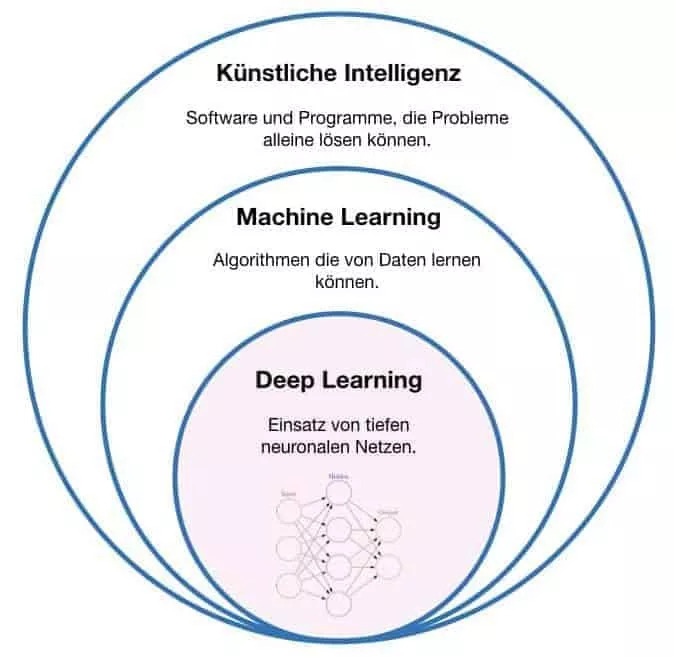
\includegraphics[width=0.9\textwidth]{deepL}
    \label{fig:deepL}
    \\
    \cite[Quelle: Vgl.][]{DeepLearning}
\end{figure}

Damit \ac{KI}-Systeme lernen, wird das sog. \enquote{maschinelle Lernen} eingesetzt. Wie in \autoref{fig:deepL} dargestellt ist, basiert dieses Verfahren auf Algorithmen die von Daten lernen können. Tiefergreifend kommt dabei das 
sog \enquote{Deep Learning}-Verfahren zum Einsatz, welches auf künstlichen neuronalen Netzen basiert~\footcite[\vglf][]{Lenzen.2020}.
Im Zuge der Digitalisierung wird unsere analoge Welt für solche informationsverarbeitenden Systeme in Form von Big Data lesbar gemacht und als Lernquelle zur Verfügung gestellt.
Trotz allem bleiben die \ac{KI}-Systeme hoch spezialisiert und können sich nicht mit der flexiblen Intelligenz der Menschen messen. Um diese Hürde zu überwinden, nähert sich die 
aktuelle \ac{KI}-Forschung wieder an die Neurowissenschaft und der menschlichen Kognition an~\footcite[\vglf][\pagef 18]{Lenzen.2020}.

\subsection{Maschinelles lernen}

Eine manuelle Erstellung von Regeln und Wissenspräsentationen, für die Verarbeitung durch \ac{KI}-Systeme, stellt einen hohen Aufwand mit nur einem begrenzten Nutzen dar~\footcite[\vglf][\pagef 4]{Matzka.2021}.
Um diesen Vorgang zu optimieren, werden nach Algorithmen und Techniken geforscht, die es \ac{KI}-Systemen ermöglichen selbständig allgemeingültige Regeln zu abstrahieren, in dem es selbständig Muster, aus einem ihm zur Verfügung stehenden
Datensatz, erkennt. Dies soll die Systeme befähigen, Vorhersagen oder Entscheidungen zu treffen, ohne explizit dafür programmiert worden zu sein. Dieser Vorgang nennt sich \ac{ML}.
Die zur Verfügung gestellten Datensätze werden auch als Trainingsdaten bezeichnet. Grundsätzlich bestehen sie aus Eingabeinformationen (Merkmalen) und Ausgabewerten (Labels oder Zielvariablen).
Besonders die Mustererkennung im hochdimensionalen Raum, durch gleichzeitige Berücksichtigung von hunderten oder tausenden Merkmalen, macht das \ac{ML} außergewöhnlich leistungsstark. Im Vergleich dazu ist es für einen Menschen
schon schwierig, drei- bis vierdimensionale Sachverhalte zu erfassen~\footcite[\vglf][\pagef 5]{Matzka.2021}.

Es existieren unterschiedlichen Arten des \ac{ML}. Beim überwachten Lernen werden dem System, wie bereits oben erwähnt, Trainingsdaten mit bekannten Eingaben und Ausgaben bereitgestellt. Daraus lernt 
das System, über eine Abbildungsfunktion, neue Eingaben für die Ausgaben abzubilden~\footcite[\vglf][\pagef 189]{Plaue.2021}. Bei der Methodik des unüberwachten Lernens werden dem System nur Eingabedaten dargeboten und es wird erwartet,
dass es von selbst Muster und Strukturen in den Daten erkennt~\footcite[\vglf][\pagef 255]{Plaue.2021}. 
Das bestärkende Lernen basiert auf der positiven oder negativen Rückmeldung auf eine bestimmte Aktion. 
Ziel ist es, dass das \ac{KI}-System auf der Grundlage der gemachten \enquote{Lernerfahrung} selbständig Vorhersagen und Entscheidungen trifft. 
Die Qualität dieser sind abhängig von der Qualität und Repräsentativität der verwendeten Daten. Auch muss der Mensch hier weiterhin evaluieren, ob die getroffenen Vorhersagen oder Entscheidungen
zuverlässig und vertrauenswürdig sind.

\ac{KI}-Systeme mit \ac{ML} werden besonders in Bereichen mit Aufgabengebieten eingesetzt, in denen Menschen Schwierigkeiten haben, diese zu lösen. Die menschliche Intelligenz wird dabei nicht ersetzt
oder simuliert, sondern komplementiert~\footcite[\vglf][\pagef 5]{Matzka.2021}.


\subsection{Big Data}

Damit {KI}-Systeme lernen können, brauchen sie sehr große Datenmengen, welche als Big Data bezeichnet werden. Dabei handelt es sich um großen Datenmengen, die in unterschiedlichen Formaten auftreten
und in verschiedenen Quellen generiert wurden. Der Autor Ralf Huss definiert Big Data als Datenmengen, die zu groß, zu komplex oder zu schwach strukturiert sind, oder sich zu schnell ändern, um mit herkömmlichen
Methoden analysiert zu werden~\footcite[][\pagef 60]{Huss.2019}. Darin liegt die große Bedeutung von Big Data, nämlich wertvolle Erkenntnisse und Muster aus Daten zu extrahieren,
bei denen herkömmliche Analysemethoden nicht ausreichen würden. Dabei können die Daten aus traditionellen Datenbanksystemen stammen oder in unstrukturierten Formaten wie Text, Audio, Video und Sensordaten vorliegen~\footcite[\vglf][\pagef 7]{Fasel.2019}.

Big Data besitzt drei Hauptcharakteristika, welche im Folgenden aufgezählt und kurz erklärt werden:

\begin{itemize}
    \item Volume - der Datenbestand bei Big Data kann enorme Ausmaße annehmen und liegt im Tera- (10\textsuperscript{12} Bytes) bis Zettabytebereich (10\textsuperscript{21} Bytes). 2008 wurden weltweit 10 Zettabytes (10\textsubscript{21} Bytes) verarbeitet~\footcite[\vglf][\pagef 61]{Huss.2019}. 
    \item Variety - der Begriff bedeutet übersetzt Vielfalt. Strukturierte Daten aus z.B. Datenbanken, semi-strukturiete Daten wie z.B. Logdateien oder Sensordaten und unstrukturierte Daten wie z.B. Textdokumente, E-Mails und Multimediadateien, werden gespeichert~\footcite[\vglf][\pagef 6]{Fasel.2019}.
    \item Velocity - der entstehende Datenstrom (Data Stream) bei Big Data wird in Echtzeit generiert und muss von entsprechend schnellen Erfassungs-, Verarbeitungs- und Analysemethoden in Echtzeit erfasst und analysiert werden~\footcite[\vglf][]{Fasel.2019}.
\end{itemize}


In einigen Quellen werden noch weitere Charakteristika für Big Data definiert, welche ebenfalls im Folgenden aufgezählt und kurz erklärt werden: 

\begin{itemize}
    \item Value - der Wert des Unternehmens soll gesteigert werden~\footcite[\vglf][]{Fasel.2019}. Dabei ist nicht unbedingt allein der monetäre Wert gemeint. In Bezug auf die Daten muss geklärt werden,
    welche Erkenntnisse aus Ihnen abgeleitet werden können, um für das verarbeitende Unternehmen einen Mehrwert darzustellen. 
    \item Veracity - da die Qualität der Daten nicht per se bekannt sind, müssen spezielle Algorithmen eingesetzt werden, um die Qualität der Resultate bzw. die Plausibilität dieser zu evaluieren. Dabei garantiert
 ein größerer Datensatz keine bessere Aussagequalität~\footcite[\vglf][]{Fasel.2019}.
\end{itemize}

Die Herausforderungen bei Big Data umfassen vor allem die Datenerfassung, -speicherung, -verarbeitung und -analyse in angemessener Zeit, Datenschutz und Datensicherheit und insbesondere die Gewährleistung der 
Datenqualität. Um diese Herausforderungen zu bewältigen, müssen Technologien wie NoSQL-Datenbanken, Cloud-Computing und verteilte System eingesetzt werden.

Big Data hat das Potenzial einen erheblichen Mehrwert für Unternehmen, Organisationen, Forschungseinrichtungen und die Gesellschaft insgesamt zu schaffen, indem es Einblicke und Erkenntnisse liefert, 
die zuvor nicht möglich waren. Es ermöglicht, bessere Entscheidungen zu treffen, Effizienz und Produktivität zu steigern und Innovationen voranzutreiben.

\subsection{Datenschutzgrundverordnung}

Die \ac{DSGVO} wurde in ihrer jetzigen Form 2018 von der Europäischen Union verabschiedet und ist ein einheitlicher Rechtsrahmen mit dem ein verantwortungsbewusster Umgang
mit den personenbezogenen Daten der Bürger der \ac{EU} sichergestellt wird~\footcite[\vglf][\pagef 2]{Voigt.2018}.
Die Verordnung stärkt vor allem die Rechte der Bürger bei der Verarbeitung ihrer personenbezogenen Daten z.B. durch Unternehmen. Personenbezogene Daten sind alle Daten, die einen Menschen
\enquote{identifizierbar} machen. Dabei reicht die bloße Möglichkeit der \enquote{Identifizierung} durch eine Kombination verschiedener Informationen, 
die für sich allein keinen Rückschluss 
auf den Betroffenen möglich gemacht hätten, aber es ermöglichen würden, aus, um als personenbezogene Daten qualifiziert zu werden~\footcite[\vglf][\pagef 14]{Voigt.2018}

Im Folgenden werden die wichtigsten Punkte der \ac{DSGVO} aufgeführt. Jeder \ac{EU}-Bürger hat das Recht zu erfahren, welche Daten über ihn gesammelt werden, warum diese Daten gesammelt werden, wie sie verwendet werden und an wen diese Daten übermittelt werden. 
Dies wird auch als Auskunftsrecht bezeichnet. Weiterführend können diese Daten durch den Bürger
berichtigt werden, falls diese falsch oder unvollständig sind. Er hat das Recht der Berichtigung, aber auch das Recht seine Daten löschen zu lassen. Ebenfalls ist es ihm möglich die 
Verarbeitung durch das Unternehmen einzuschränken, oder dieser im gesamten zu widersprechen~\footcite[\vglf][\pagef 200]{Voigt.2018}. Des Weiteren hat er das Recht der Datenübertragbarkeit. Hierbei müssen die Daten der
betroffenen Person in einem gängigen maschinenlesbaren Format übermittelt werden oder diese einem anderen Unternehmen bereitstellen.
Personenbezogene Daten dürfen nicht ohne die Einwilligung der betroffenen Person erhoben oder verarbeitet werden. Dabei muss die Einwilligung freiwillig, spezifisch, informiert und
unmissverständlich sein.
Unternehmen müssen \enquote{Datenpannen}, z.B. die Offenlegung von personenbezogenen Daten, innerhalb von 72 Stunden an eine Datenschutzbehörde melden~\footcite[\vglf][\pagef 86]{Voigt.2018}.
Die \ac{DSGVO} ist noch deutlich umfangreicher und hat beträchtliche Auswirkung auf Unternehmen, besonders solche, die große Mengen an personenbezogenen Daten sammeln und verarbeiten.
Sie dient vor allem dem Schutz der Privatsphäre der \ac{EU}-Bürger.
Verstöße gegen die DSGVO können zu erheblichen Strafen führen. Unternehmen sind daher angehalten, ihre Datenverarbeitungsprozesse sorgfältig zu prüfen und zu verwalten~\footcite[\vglf][\pagef 85]{Voigt.2018}.


\section{Chancen und Risiken von künstlicher Intelligenz} \label{Chancen und Risken von KI}
Die Möglichkeiten der Anwendung von künstlicher Intelligenz sind sehr vielfältig. Sie bergen sowohl Chancen als auch Risiken mit sich. 
Infolgedessen sollen verschiedene Anwendungsmöglichkeiten von KI - Systemen dargestellt werden und auf ihre Chancen und Risiken hin untersucht werden. 

\subsection{Chancen beim Einsatz von künstlicher Intelligenz}
\subsubsection{intelligente Assistenten}
Das Unternehmen IBM hat maßgeblich den Begriff \enquote{Cognitive Computing} geprägt. Der Begriff bezieht sich auf Systeme,
die skalierbar lernen und durch zielgerichtete Schlussfolgerungen mit Menschen interagieren können.
Diese Systeme können auf komplexe Fragestellungen mit Hypothesen, logischen Argumenten und Empfehlungen antworten~\footcite[\vglf][\pagef 23]{Scherk.2017}.
Der deutsche Digitalverband Bitkom zählt zu den Kernmerkmalen eines solchen Systems die \textbf{Adaptivität} sich an ein verändertes Umfeld anzupassen, sowie die 
\textbf{Interaktivität} mit Nutzern in Interaktion zu treten und dabei durch \textbf{Iterativität} Ziele und Probleme im Dialog zu präzisieren. Dabei ist es in der Lage
aus Informationen, aus vielen unterschiedlichen Quellen, die richtigen Schlüsse zu ziehen, die sog \textbf{Kontextualität}~\footcite[\vglf][\pagef 23]{Scherk.2017}.

Kognitive System ermöglichen für den Anwender eine \enquote{persönliche} Interaktion in natürlicher Sprache. Dabei ziehen die Systeme aus strukturierten und unstrukturierten
Daten, wie Text, Bild oder Sprache, Informationen, z.B. was einem Nutzer wichtig ist und gestalten durch das Hinzufügen von Details wie Stimmung und Umgangston eine natürliche 
Kommunikation. 
Explorative kognitive Systeme können dabei eigenständige Hypothen entwickeln, eine komplette Darstellung der wissenschaftlichen Literatur und gesellschaftlichen
Diskussion bereitstellen oder die Konsequenzen einer Absicht erörtern~\footcite[\vglf][\pagef 24]{Scherk.2017}.

Durch die Verwendung solcher intelligenter Systeme steigen die Kenntnisse und Kompetenzen der Benutzer, aufgrund des Umfangs und der deutlich schnelleren Verfügbarkeit
von Wissen und dadurch steigenden Lernmöglichkeiten. Das Beispiel der Verbreitung von medizinischem Wissen verdeutlicht dies. 1950 
dauert es schätzungsweise ungefähr 50 Jahre, um das Wissen weltweit zu verdoppeln. 1980 waren es nur noch sieben Jahre und 2015 nur noch drei Jahre.
Die Systeme können Unternehmen und Organisationen helfen, mit der stetigen Entwicklung mitzuhalten und Ihre Leistungen zu verbessern~\footcite[\vglf][\pagef 25]{Scherk.2017}.

Im Einzelhandels- und Dienstleistungsgewerbe ermöglichen intelligente Assistenten bessere Produkte und Dienstleistungen durch die Interaktion mit den Kunden 
und die daraus resultierenden Schlussfolgerungen über dessen Vorlieben und Kaufverhalten.
Als Beispiel dient hier \enquote{H\&M Home Stylist}, ein Chatbot von der Firma H\&M, welcher den Kunden bei der Einrichtung Ihres Zuhauses unterstützt. Der Chatbot 
fragt den Kunden nach seinen Vorlieben und basierend auf seinen Antworten sucht der Chatbot passende Produkte für ihn aus. Mit Einführung des \enquote{H\&M Home Stylist}
wurde die Kundenzufriedenheit gesteigert und der Umsatz des Unternehmens erhöht~\footcite[\vglf][\pagef 53]{Robot.2023}.

Ebenfalls werden durch die Interaktion mit intelligenten Systemen neue Daten generiert, die wiederum ausgewertet werden können und aufgrund neu gefundener Muster neue Handlungshypothesen
ermöglichen.

Der immer stetig wachsende Einsatz von intelligenten Assistenten wird zahlreiche Arbeitsprofile, insbesondere von Wissensarbeitern, verändern. Es wird sich eine Arbeitsteilung 
zwischen dem kognitiven System und Menschen entwickeln, indem sie kooperieren. Dadurch entsteht eine Kombination aus den jeweiligen Stärken der beiden Entitäten, z.B. indem
die kognitiven Systeme die menschliche Kreativität in Innovationsprozessen verstärken~\footcite[\vglf][\pagef 25]{Scherk.2017}.
Ein Beispiel einer solchen Kooperation ist eine Investmentfirma aus Hongkong. Diese hat einem kognitiven System den Status eines Vorstandsmitgliedes übertragen. Ohne die Zustimmung
des Systems werden keine Investitionen mehr abgesegnet~\footcite[\vglf][\pagef 25]{Scherk.2017}.

\subsubsection{Robotik}
Die bereits erwähnte Kooperation ist besonders in der Robotik zu erkennen. Allein in Deutschland kommen ca. 1.8 Industrieroboter in der Arbeitswelt zum Einsatz und erleichtern
den Arbeitsalltag vieler Menschen. Allerdings soll es im folgenden Kapitel um sog. soziale Roboter gehen. In Deutschland sind künstlichen Gehilfen noch eine Ausnahmeerscheinung,
während diese in den USA und Japan bereits Alltag ist. Dort sind Wachroboter zur Überwachung der Besucher in Einkaufszentren, Flughäfen oder Restaurants und autonome Pizzaboten im Versuchsstadium im Einsatz. Ebenfalls werden Roboter in 
Altenheimen zur Rehabilitation und Therapie eingesetzt. Die Spannweite reicht dabei von einer Terminerinnerung über Nachhilfe bis hin zum Einsatz als Polizeiassistenten.
Auch können Sie als Kinderspielzeug, Babysitter oder sogar als ein Ersatz für eine persönliche Beziehung eingesetzt werden~\footcite[\vglf][\pagef 107]{Heinrichs.2022}.
Es ist davon auszugehen, dass die Interaktion mit sozialen Robotern in Zukunft eine Selbstverständlichkeit erreicht, die den Umgang mit dem Smartphone gleichzusetzen ist.

Grund für diesen Erfolg ist vor allem die Tatsache, dass diese künstlichen Gehilfen manche Arbeiten gleichwertig oder besser verrichten als ihr menschliches Pendant, aber auch
Arbeiten verrichtet, die für Menschen unliebsam sind. 
Vielen Menschen profitieren auch vom Umgang mit Robotern, insbesondere bei Therapien von Menschen, die den Kontakt zu Menschen meiden z.B. Autisten. Als weiteres Beispiel für die Arbeitserleichterung durch künstliche Gehilfen lassen sich 
Pflegeroboter anführen, die die physischen Lasten des meist weiblichen Personals reduzieren~\footcite[\vglf][\pagef 108]{Heinrichs.2022}.

\subsubsection{Autonomes Fahren}
Autonomes Fahren verspricht vor allem die Sicherheit im Straßenverkehr zu erhöhen, indem die Anzahl der Verletzten und Verkehrstoten reduziert wird. Zum aktuellen Zeitpunkt
gibt es bereits unzählige Fahrassistenzsysteme, wie z.B. automatische Einparkassistenten, die vor allem den Fortschritten in der Sensorik und im \ac{ML} zu verdanken sind.
Unfälle können bspw. vermieden werden, indem Gefahrensituationen im Voraus erkannt werden, indem auf Grundlage der Projektion von Bewegungspfaden von Verkehrsteilnehmern die Risikolage
von Kollisionen analysiert werden.
Bereits jetzt können selbstfahrende Autos mehrere tausend Kilometer unfallfrei zurücklegen, ohne die Notwendigkeit eines menschlichen Eingreifens~\footcite[\vglf][\pagef 29]{Scherk.2017}.

Die \ac{KI} wird einen wesentlichen Beitrag bei der Optimierung von Verkehrsflüssen leisten. Im Personen- und Warenverkehr können Staus vermieden werden, indem Verkehrsströme aufeinander 
abgestimmt werden und so die Verkehrsinfrastruktur entlasten. Auch können freie Kapazitäten erkannt und ausgenutzt werden, indem die Grünphasen von Ampeln an das momentane
Verkehrsaufkommen angepasst werden~\footcite[\vglf][\pagef 178]{Wittpahl.2018}. Diese Verbesserungen wären ein großer Schritt in Richtung umweltfreundliche Mobilität, da zum einen 
die Emissionen verringert und zum anderen der Verkehrsfluss optimiert werden würde. Auch andere ressourcenschonende Lösungen, wie die intelligente Ladezyklen Steuerung in der Elektromobilität
führt zu einer Verlängerung der Lebensdauer, bei gleichzeitiger Erhöhung der Reichweite~\footcite[\vglf][\pagef 178]{Wittpahl.2018}.
Für neue Mobilitätsformen wie autonome Flugtaxis oder Logistik-Drohnen wird zukünftig der Einsatz von KI ebenfalls eine entscheidende Rolle spielen~\footcite[][\pagef 178]{Wittpahl.2018}.

\begin{figure}[H]
    \centering
    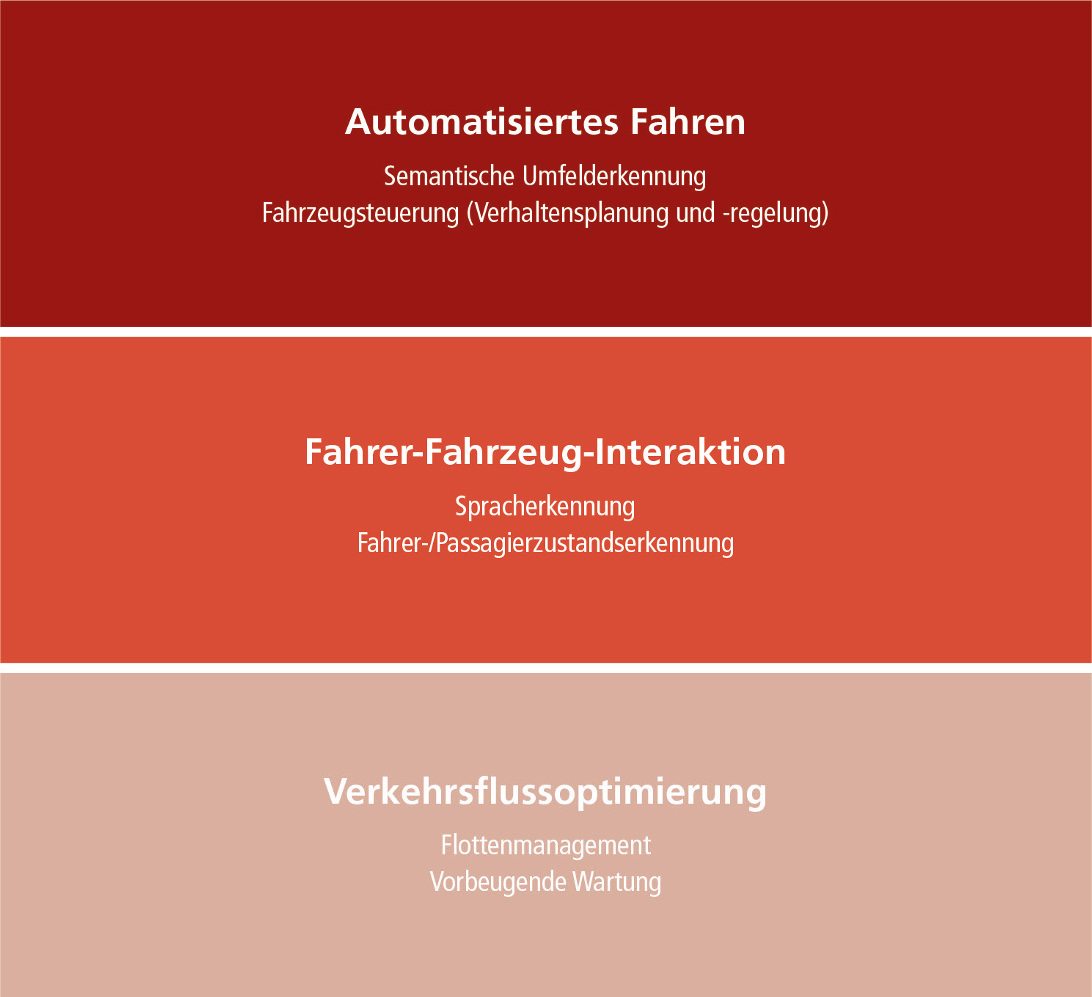
\includegraphics[width=0.8\textwidth]{AF} 
    \caption[Überblick der Anwendungsbereiche der KI für das automatisierte \mbox{Fahren}]{Überblick der Anwendungsbereiche der KI für das automatisierte \mbox{Fahren}\footnotemark}
    \label{fig:af}
\end{figure}
\footnotetext{\cite[\vglf][\pagef 179]{Wittpahl.2018}}

Wie in \autoref{fig:af} zu sehen ist, hat \ac{KI} neben dem automatisierten Fahren und der Verkehrsflussoptimierung auch noch die Aufgabe der Fahrer-Fahrerzeug-Interaktion. Der Mensch 
gibt immer mehr Verantwortung und Aufgaben an die \ac{KI} ab. Das hat den positiven Effekt, dass diese immer mehr Trainingsdaten erhält und sich dadurch stetig verbessert.
Hierdurch wird das Vertrauen in das autonome Fahren steigen und die Mobilität sich weiter wandeln~\footcite[\vglf][\pagef 188]{Wittpahl.2018}.

\subsubsection{Gesundheitsweisen}

Das Gesundheitsweisen profitiert besonders von der modernen Entwicklung in der \ac{KI}-Forschung. \ac{KI} kann in der medizinischen Forschung, bei der Diagnose sowie Behandlung 
von Krankheiten eingesetzt werden. Auch die Verwaltung von Gesundheitsdaten kann von der \ac{KI} übernommen werden~\footcite[\vglf][\pagef 177]{Robot.2023}.

Durch die sehr gute Musterkennung in großen Datensätzen können \ac{KI}-Systeme besonders vorteilhaft in der Medizin eingesetzt werden. Sie können die erkannten Muster mit
der Krankengeschichte des Patienten abgleichen und so Erkenntnisse hervorbringen, die ein menschlicher Arzt mit dem menschlichen Auge und der menschlichen kognitiven Limitierung nicht 
erkennen würde~\footcite[\vglf][\pagef 392]{Buchkremer.2020}. Sie sind auch in der Lage, bei der Diagnose und bei der Behandlung von Krankheiten zu helfen, 
da sie imstande sind, genetische Informationen eines Menschen zu analysieren oder seine medizinischen Bilder auszuwerten~\footcite[\vglf][\pagef 177]{Robot.2023}.

Es ist davon auszugehen, dass Ärzte in der näheren Zukunft nicht mehr allein agieren werden, sondern Sie ein Dreiergespann aus Arzt, Patient und Maschine bilden werden. 
Das hat den Vorteil, dass der Arzt bei seiner Diagnostik durch ein \ac{KI}-System unterstützt wird und so fehlerhafte Diagnosen verhindert werden können, denn ungefähr 
20-30\% aller Diagnosen im ambulanten Bereich sind zurzeit falsch~\footcite[\vglf][\pagef 392]{Buchkremer.2020}.

Aber auch das Gesundheitsweisen hat die Chance, einen positiven Einfluss auf die \ac{KI}-Entwicklung zu nehmen, indem eine gemeinsame Kooperation entsteht, in der offen kommuniziert wird.
Desto mehr die \ac{KI}-Entwicklung in den medizinischen Prozess eingebunden wird, umso mehr könnte das Gefühl entstehen, dem Gemeinwohl zu dienen und die eigenen
Interessen zurückzustellen. Dies würde einen positiven Effekt für alle Bereiche erwirken. Auch könnte der externe Einfluss auch eine Minimierung von 
Sicherheitsrisiken nach sich ziehen, da alle Teilnehmer altruistisch motiviert wären~\footcite[\vglf][\pagef 392]{Buchkremer.2020}. 
Wichtig wäre hierbei allerdings, dass das Ganze innerhalb der Grenzen des \ac{DSGVO} geschehen sollte, um die Sicherheit und die Persönlichkeitsrechte der Patienten zu wahren.

\subsection{Risiken beim Einsatz von künstlicher Intelligenz}
\subsubsection{Arbeitswelt}
Eine der größten Anwendungsbereiche von \ac{KI}-Systemen stellt der Wirtschaftssektor dar z.B. werden sie eingesetzt für die Rekrutierung von Personal und den Verkauf von Gütern zu optimieren oder um
Arbeitsprozesse in quantitativer und qualitativer Hinsicht zu verbessern. Der Einsatz von solche System ist auch mit der Hoffnung verknüpft, eine umfangreiche
Automatisierung aller Wirtschafts- und Arbeitsprozesse zu realisieren~\footcite[\vglf][\pagef 127]{Heinrichs.2022}.

Der Konsens vieler Autoren ist dabei gleich, dass es in der Zukunft viel weniger Bedarf für menschliche Arbeit gibt, besonders in Bereichen in dennen es viele
sich wiederholende und einfache Aufgaben gibt wie z.B. in der Produktion oder der Buchhaltung~\footcite[\vglf][\pagef 130]{Robot.2023}.
Das betrifft vorallem Bereich, in dennen niedrig qualifizierten Arbeitnehmern arbeiten. Besser qualifizerte Arbeitnehmen werden weiterhin 
benötigt, um die \ac{KI}-Systeme zu überwachen. Dies kann zu einer sozialen Ungleichheit führen, da Arbeitnehmer mit geringer Bildung 
und Qualifikation benachteiligt werden~\footcite[\vglf][\pagef 130]{Robot.2023}. Damit dieser Effekt gedämpft wird, müssen Arbeitnehmern
kontinuierlich geschult werden, um sie an den sich stetig verändernden Arbeitsmarkt anzupassen.
Dennoch werden Menschen, die keinen bis schlechten Zugang zu Bildung haben und nur wenig finazielle Ressourcen besitzen, ins Hintertreffen geraten. 
Unternehmen, Regierungen und Arbeitnehmern müssen sich auf die anstehenden Veränderungen einstellung und diesen Effekt durch eine besseren und leichtern
Zugang zu Bildung und Schulungen abfedern~\footcite[\vglf][\pagef 130]{Robot.2023}.

Je schneller die Automatisierung vorranschreitet, desto mehr Arbeitsplätze fallen weg. Der Einsatz von \ac{KI}-System schafft zwar auch neue hochqualifizerte 
Arbeitsplätze und senkt die Produktionskosten, aber die daraus entstehende Nachfrage durch automatisierten Prozess abgedeckt wirdd.
Innerhalb Amazons Lagerhalten arbeiten bereits mehr als 100.000 Roboter~\footcite[\vglf][\pagef 49]{Kipper.2020}.

Im Verlauf der Zeit wird die \ac{KI} in immer mehr Berufsfelder Einzug halten, auch in kogntive Berufe wie z.B. den Journalismus. Die Menschheit muss sich 
auf Lange sicht Wege und Möglichkeiten suchen, wie sie das gesellschaftliche Leben ohne Arbeit gestalten kann.
    
\subsubsection{Überwachung, soziale Kontrolle und Diskriminierung}

Big Data stellt ein großes Machtpotenzial dar, da durch die Datenherbung von Unternehmen und Regierungen unzählige Daten von Bürgern erfasst wurden. Die systematische 
Auswertung dieser Daten ermgölich es \ac{KI}-System dieses Machtpotenzial auszuschöpfen.
Als negatives Beispiel dient die Volksrepublik China. Unter dem Deckmantel eines Gesundheitsprogramms wurden in den Jahren 2016 bis 2017 biometrische Daten aller
Bewohner der Provinz Xinjiang gesammelt. Die Daten umfassen Blutgruppe, Irisscans, Stimmaufnahmen und DNA. Im Jahr 2019 wurde eine Datenbank mit den Daten von 2,5 Millionen
Einwohnern Xinjiangs entdeckt, die aufgrund der vorangegangen Datensammlung, mit modernster Überwachungstechnologie überwacht wurden~\footcite[\vglf][\pagef 33]{Kipper.2020}.
Weiter hat China 2020 ein Sozialkreditsystem eingeführt, welches ohne Gesichterkennung, Spracherekknung und der massenhaften Erfassung und Verarbeitung von Daten durch
\ac{KI}-Systeme nicht möglich wäre. Dieses System belohnt vermeindlich \enquote{gute} Bürger mehr Privilegien. Wohingehen \enquote{unsoziales Verhalten} zu einer Verringerung der
Sozialpunkte des Bürger führt. Dies hat für Ihn negative Auswirkungen, die von längeren Wartezeiten bei Behörden, bis hin zu Ablehnung bei Ticketkäufen für den öffentlichen Verkehr
reichen können. Der Fortschritt in der \ac{KI}-Forschung wird immer mehr Möglichkeiten eröffnen, Menschen zu kontrollieren~\footcite[\vglf][\pagef 33]{Kipper.2020}.

Auch in der westlichen Welt, wird die Auswertung von Daten durch \ac{KI}-Systeme verwendet, um Menschen zu kontrollieren, vornehmlich allerdings im privaten Sektor durch Werbung.
Über die Suchen bei Online-Suchmaschinen, aufrufen von Webseiten, oder Gesprächen in Reichweise eines digital Assisten wie z.B. Amazons \enquote{Alexa} wird den Bürgern
gezielt Werbung angezeigt. Künstliche neuronale Netze finden dafür bestimmte Attribute in Korrelation~\footcite[\vglf][\pagef 33]{Kipper.2020}.
Aus den resultierenden Daten kann auch abgeleitet werden, welche Schwächen ein Mensch besitzt, z.B. Online-Glückspiel. Die Gefahr, dass durch die wiederholte Anzeige von 
Glückspielwerbug, aufgrund eines einmaligen Suchvorgangs, ein Suchtverhalten ausgelöst wird, ist nicht unwahrscheinlich.
Aber es können auch Aussagen über das Kaufverhalten und der Zahlungsbereitschaf von Kunden getroffen werden. So finden sich in persönlicher Werbung oftmals deutlich
teurere Preise als allgemeiner Werbung.
Wenn Unternehmen auf der Basis immer größerer Datenmengen und immer besserer KI Konsumentenverhalten immer präziser vorhersagen und damit steuern können, 
könnte das zu einem gewaltigen Machtgefälle zu Ungunsten der Verbraucher führen~\footcite[\vglf][\pagef 35]{Kipper.2020}.


\subsubsection{Autonome Waffensysteme}

Bereits seit die ersten Schritte in der \ac{KI}-Forschung getan waren, war diese eng mit dem Militär verbunden. Der Militär-Apparat verwendet bereits Software, die Luftbilder auswerten kann,
über Exoskelette, die Soldaten mehr Kraft verleihen, bis hin zu Drohnen und zu System zur Kontrolle von Waffensystem, aus der \ac{KI} und Robotik.
In der Neuzeit kamen auch \enquote{Cyberschlachtfelder} hinu, wo um die Kontrolle von zivielen und militärischen Computersystem gekämpft wird~\footcite[\vglf][\pagef 86]{Lenzen.2020}.

Nach einem Bericht des Futere of Life Institute existieren momentan Weltweit 284 Waffensystem die autonom agieren können. Größtenteils handelt es sich dabei um Raketen,
die eine eigenständige Ziielsuche besitzen. Die Vorfilterung von Informationen und das eigenständige treffen von Entscheideung stellt dabei einen strategischen Vorteil dar. 

Der Mensch bekommt nur noch vorgefilterte Information durch ein Computersystem, was aufgrund der schieren Menge an Daten nicht anders möglich st. Letzendlich trifft dieser
die Entscheidung, allerdings stellen Froscher sich die Frage, inwieit ein Mensch aufgrund der vorgefilterten Informationen durch ein \ac{KI}-System wirklich relevant entscheiden~\footcite[\vglf][\pagef 88]{Lenzen.2020}.
zieht man alles in Betracht, so sind Szenarien vorstellbar, in dennen \ac{KI} gesteuerte Schwärme von Drohnen per Gesichtserkennung gezielt nach Personen suchen und diese liqudieren~\footcite[\vglf][\pagef 28]{Kipper.2020}.
Ebenfalls entsteht eine Verantwortungslücke, da eine \ac{KI} in keinster Weise zur Rechenschaft gezogen werden kann, und der menschlichte Akteur seine Verantwortung auf die 
\ac{KI} überträgt~\footcite[\vglf][\pagef 153]{Heinrichs.2022}.
Ihr können zwar die Regel des Völkerrechts einprogrammiert werden, dennoch empfindet sie keine Empathie oder besitzt Emotionen.
Autonome Waffensystem können auch die Hemmschwelle der beteiligten Parteien zur Konflikteskalation senken, da der Einsatz von autonomen Waffensystemen nicht den Einsatz 
von menschlichen Soldate, auf dem Schlachtfeld, benötigt.
Aufgrund der übermenschlichen Geschwindigkeit der Datenverarbeitung von solchen System, könnte eine solche Situation eskalieren und nicht mehr kontrollierbar durch den Menschen werden.
Eine fatale Situation bei der enormen Zerstörungskraft solcher Systeme.

Ein Vorteil ist nicht von der Hand zu weisen, durch den Einsatz von autonomen Waffensystem, wird die Anzahl der menschlichen Beteiligten an einem Kampfgeschehen minimiert und 
somit auch die Opferzahlen~\footcite[\vglf][\pagef 30]{Kipper.2020}.
\newpage
\section{Zukünftige Herausforderungen}\label{Herausforderungen}

Mit dem Einsatz von \ac{KI} entstehen viele Herausforderungen für die Gesellschaft. Sie hat bereits und wird immer mehr Einfluss auf soziale, politische und ökonomische Systeme haben.
Viele Wissenschaftler befürchten, dass der Mensch sich in nahen Zukunft einen Wettlauf mit einer \enquote{Superintelligenz} liefern wird und diesen verlieren wird,
da Maschinen und \ac{KI} im speziellen viel schneller adaptiert und reagiert und der Mensch aus evolutionärer Sicht nicht mithalten kann. Mit diesem Hintergrund ist 
Notwendigkeit einer Außereinandersetzung mit den ethischen Dimensionen von \ac{KI} entstanden~\footcite[\vglf][\pagef 239]{Wittpahl.2018} und weiter anhaltend, da \ac{KI}s
immer tiefer in gesellschaftliche Thematiken vordringen und keinerlei Beschränkungen unterliegen. Das verändern von Wertschöpfungsprozessen, privater Kommunikation und 
besonders der zwischenmenschlichen Interaktion erfordert ethische Grenzen und Prinzipien. Der Einfluss der \ac{KI} wird noch deutlicher wachsen, 
wenn eine sich selbstgestaltende und fortentwickelnde, eine sog. starke \ac{KI}, Realität wird. Es werden dringend die Antworten auf die Fragen gesucht, was \ac{KI} mit
unserer Gesellschaft macht und wie sie unser momentanes Leben und Arbeitswelt weiter verändert wird~\footcite[\vglf][\pagef 239]{Wittpahl.2018}.

Algoithmen, die große Mengen an Daten analyiseren und nach Mustern suchen, eigenen sich sehr gut den Menschen zu erforschen. Die Daten, welche die intelligenten System von den 
Nutzern benötigen, um Ihnen das Leben zu erreichen, machen die Nutzer Zeitgleich durchsichtig. Unternehmen verkaufen diese Daten. Der Mensch wird zum Produkt~\footcite[\vglf][\pagef 114]{Lenzen.2020}.
Zum Schutz dieser Daten und der Privatsphäre wurde die \ac{DSGVO} in der \ac{EU} verabschiedet. Weitergehend müssen Mechanismen entworfen werden, die sicherstellen, dass
\ac{KI}-Systeme sicher und vertrauenswürdig sind. 
Denn diese System können auch zu Verzesserung und Vorurteilen führen, abhänging von den Ihren vorliegenden Daten. Kein Mensch darf durch \ac{KI}-Systeme diskriminiert werden.
Allerdings ist dies äußerst diffizil, da \ac{KI}-Systeme äußerst komplexe Entscheiden treffen, die für Menschen schwer zu verstehn und zu erklären sind. Es fehlt an 
Erklärbeit und Transparenz. Dies ist besonders priker in Bereich in dennen es um Menschenleben geht, wie z. B. in der Medizin. Die Entscheidungen müssen für den Menschen 
nachvollziehbar sein, nach welchen Kriterien diese entstanden sind~\footcite[\vglf][\pagef 240]{Wittpahl.2018}.
Daraus resultiert die Fragestellung, inwieweit die Menscheit den \ac{KI}-System die autonome Entscheidungsmöglichkeit überlässt. Es müssen Regularieren evaluiert werden,
die klären wer für die Entscheidungen eines \ac{KI}-System die Verantwortung übernimmt, z. B: auch beim autonomen Fahren im Falle eines Unfalls. Wie oben bereits erwähnt müssen ehtische Rahmenbedingungen geschaffen werden, 
die die Autonomie von \ac{KI}System regelt und eine klare Verantwortun für Ihre Entscheidungen und Handlungen festlegen~\footcite[\vglf][\pagef 35]{Robot.2023}.

Ein möglicher weg ist der der Aufbau von Transparenz und Überwachungsstrukturen, von Standards und Sanktionsmustern. Dies wird von vielen Wissenschaftlern als Grundvorrausetzung
für einen ethische verantwortungsvolle Nutzung angesehen~\footcite[\vglf][\pagef 243]{Wittpahl.2018}. Für den Umgang mit \ac{KI} braucht es Vertrauen, welche nur durch den
Souveränität und Kompetenz erreicht werden kann. Ein erster SChritt wurde dahingehnd schon unternommen. Initiativen wie AINOW oder OpenAI versuchen globale Standards für \ac{KI}-Systeme
etablieren um sie zu demokratisieren und für alle Menschen zugänglich zu machen. Große Unternehmen wie Google, Apple, Facebook und Amazon, stellen Ihre KI-Tools als 
Open-Source zur Verfügung, um die KI-Souveränität zu fördern und im gleichen Zuge von der Schwarmintelligenz zu profitieren. In Europa wird über eine spezielle
Forschungseinrictung für KI nachgedacht, an dennen das Wissen und die Kompetenzen zentral gebündelt werden~\footcite[\vglf][\pagef 243]{Wittpahl.2018}.

Daran ist gut gelegen, denn einfach den Stecker zu ziehen, ist nicht mehr Möglich. Die \ac{KI} muss nach ihren eigenen, von Menschen geschaffenen, 
Ethik handelnu~\footcite[\vglf][\pagef 244]{Wittpahl.2018} und der Mensch muss ihr vertrauen können.

% irgendwo einfügen ggf

Sobald \ac{KI} ein Teil unserer Gesellschaft ist, kann sie diese auch Beeinflußen, im positiven wie im negativen Sinne z. B. droht ein dringender Handlungsbedarf
im niedrig Qualifizierten Arbeitssektor. Viele Menschen könnten Ihren Arbeitsplatz verlieren. Die Menschheit muss sich neue Wege und Möglichkeiten suchen Ihr Leben zu 
gehalten. \ac{KI} wird das Leben, wie wir es heutzutage führen, stark verändern. Es ist vorstellbar, das Menschen Ihren Alltag ohne Arbeit gestalten werden. Dies ist eine
überaus umfangreiche Herausforderung.

% S. 265 für Ausblick dann ggf.

\newpage
\section{Fazit}\label{Fazit}
Die vorliegende Arbeit hat sich mit der Thematik \enquote{Die Chancen und Risiken beim Einsatz von künstlicher Intelligenz in der modernen Gesellschaft und die damit verbundenen Herausforderungen}
beschäftigt. Dabei wurde herausgearbeitet, welche Chancen und Risiken der Einsatz von \ac{KI} in unserer heutigen Gesellschaft umfasst und welche zukünftigen Herausforderungen
auf die Menschheit zukommen.
Bezüglich der Chancen des Einsatzes von \ac{KI} lässt sich resümierend feststellen, dass es vielfältige Möglichkeiten gibt. Intelligente Assistenten werden die Menschen immer mehr in ihrem
alltäglichen Leben begleiten. Der Mensch wird eine Kooperation mit den intelligenten Assistenten eingehen, in der die jeweiligen Stärken optimal ausgenutzt werden. 
Im gleichen Zug werden soziale Roboter einen immer höheren Anteil in unserem Leben einnehmen. Sie übernehmen Arbeiten, in dennen Sie besser sind als Menschen, oder die Menschen
ungerne Verrichten. Sie werden zum normales Bild im modernen Alltag.
Weiterhin wird der Verkehrsfluss optimiert, durch eine \ac{KI} gesteuerte Verkehrsinfrastruktur, mit dem wesentlichen Vorteil, dass es weniger Verkehrstote gibt und die Sicherheit
im Straßenverkehr deutlich erhöht wird. Das ganze wird auch einen positiven Effekt auf die Umwelt haben, durch andaurende Optimierung z. B. die Reichweite von Elektrofahrzeugen 
erhört wird, bei sinkendem Energieverbrauch.
Durch die hervoragende Musterkrennung wird \ac{KI} auch immer mehr im Gesundheitweisen eingesetzt, in der medizinischen Forschung und bei der Behandlung von Krankheiten. 
Dabei werden sie mit menschlichen Ärzten zusammenarbeiten.
Hinsichtlich der Risiken beim Einstz von \ac{KI} lässt sich feststellen, dass diese einen großen Einfluss auf den Arbeitsmarkt haben wird. Es besteht die Gefahr, dass auf kurze Sicht,
besodners Arbeitstellen in Gefahr sind, die eine niedrige Qualifikation erfordern. Auf lange Sicht, wird sich \ac{KI} auch auf kogntive Berufe erstrecken. Die Gesellschaft wird nach Möglichkeiten
suchen müssen, ein Leben ohne Arbeit zu führen.
Auch besteht die Gefahr das \ac{KI} zur Überwachung, soziale Kontrolle und Diskriminierung eingesetzt wird. Das chinesische Sozialkredit-System ist ein modernes Beispiel dafür. Auch findet es
in unserem Alltag statt, indem wir maßgeschneiderte Werbung erhalten oder in Städten oder an Flughäfen per Gesichtserkennung überwacht werden.
Ein ganz großes Punkt beim Einsatz von \ac{KI} sind autonome Waffensysteme. Dabei stellt sich die Frage der Verantwortung beim Einsatz. Vorallem singt die Hemmschwelle zur Konflikteskalation, da es keine Menschliche beteiligung gibt.
Aufgrund der enormen Datenverarbeitungskapazitäten können solche Situationen schnell eskalieren und durch den Menschen nicht mehr kontrollierbar werden, was eine verherrende
Auswirkungen haben könnte.
Die darauf resultierenden Herausforderungen, machen deutlich, dass wir uns vorallem mit den ethischen Dimensionen des Einsatzes von \ac{KI} auseinander setzen und Reglen aufstellen müssen.
Durch die enorm hohe Verabeitungsrate werden die getroffener Entscheidungen einer \ac{KI} für den Menschen nicht mehr nachvollziehbar, was besonders in Bereichen sehr gefährlich ist, in dennen
Menschen davon betroffen sind. 
Auch muss die Privatsphere der Menschen beschützt werden, damit solche \ac{KI} nicht alles verarbeiten und darauf Schlussfolgerungen ziehen, die für den einzelnen Problembehaftet sind. Ein erster
Schritt erfolgte in der verabschiedung der \ac{DSGVO} oder in der evualuierung globaler Standards für den Umgang.
Alles in allem lässt sich sagen, dass der Erfolg von \ac{KI} ein ethisches Regelwerk vorraussetzt. Wenn dies gegeben ist, lassen sich die Stärken von \ac{KI} entfalten und der Missbrauch
verhindern. 
\newpage
\section{Ausblick} \label{Ausblick}

Es ist nicht von der Hand zu weisen, dass \ac{KI}-Tools eine immer wichtigere Rolle in der Zukunft in unserer Gesellschaft spielen werden. Sie werden unser Leben in vielen Bereichen
verbessern. Dabei muss aber die Geselllschaft sicherstellen, dass sie die Chancen und Herausforderungen, die mit der Nutzung von {KI} verbunden sind sorgfältig abwägen
und verantwortungsbewusst handeln, um die Vorteile optimal zu nutzen und die Risiken zu minimieren.~\footcite[\vglf][\pagef 57]{Robot.2023} Die zentrale Frage von Organisationen,
Gesellschafft und Individuen, wird sein, welche Entscheidungen sie an die \ac{KI} abgeben können und welche nur vom Menschen getroffen werden dürfen.~\footcite[\vglf][\pagef 274]{Wittpahl.2018}
In Zukunft wird \ac{KI} ein spannendes und umstrittenes Thema nicht nur bei technischen Fragen, sondern auch bei ehtischen, sozialen und politischen Implikationen.~\footcite[\vglf][\pagef 149]{Robot.2023}
Regierungen, Unternehmen, Forschungseinrichtungen und die Gesellschaft ingesamt, werden gemeinsam die Entwicklung von \ac{KI} begleiten. Ethikkommissionen und Regulierungsbehörden müssen sicherstellen,
dass ehtische und gesetzliche Vorgaben eingehalten werden.~\footcite[\vglf][\pagef 149]{Robot.2023}
Bei allem vorangegenan ist festzuhalten, dass \ac{KI} auch in Zukunft keine gesellschaftlichen Probleme lösen und uns auch keine politischen Entscheidungen abnehmen wird.
Sie wird uns als Gesellschaft aber helfen, bessere Entscheidungen zu treffen. Diese Hilfe können wir gut gebrauchen.~\footcite[\vglf][\pagef 124]{Lenzen.2020}



%-----------------------------------
% Literaturverzeichnis
%-----------------------------------
\newpage

% Die folgende Zeile trägt ALLE Werke aus literatur.bib in das
% Literaturverzeichnis ein, egal ob sie zietiert wurden oder nicht.
% Der Befehl ist also nur zum Test der Skripte sinnvoll und muss bei echten
% Arbeiten entfernt werden.
%\nocite{*}

%\addcontentsline{toc}{section}{Literatur}

% Die folgenden beiden Befehle würden ab dem Literaturverzeichnis wieder eine
% römische Seitennummerierung nutzen.
% Das ist nach dem Leitfaden nicht zu tun. Dort steht nur dass 'sämtliche
% Verzeichnisse VOR dem Textteil' römisch zu nummerieren sind. (vgl. S. 3)
%\pagenumbering{Roman} %Zähler wieder römisch ausgeben
%\setcounter{page}{4}  %Zähler manuell hochsetzen

% Ausgabe des Literaturverzeichnisses

% Keine Trennung der Werke im Literaturverzeichnis nach ihrer Art
% (Online/nicht-Online)
%\begin{RaggedRight}
%\printbibliography
%\end{RaggedRight}

% Alternative Darstellung, die laut Leitfaden genutzt werden sollte.
% Dazu die Zeilen auskommentieren und folgenden code verwenden:

% Literaturverzeichnis getrennt nach Nicht-Online-Werken und Online-Werken
% (Internetquellen).
% Die Option nottype=online nimmt alles, was kein Online-Werk ist.
% Die Option heading=bibintoc sorgt dafür, dass das Literaturverzeichnis im
% Inhaltsverzeichnis steht.
% Es ist übrigens auch möglich mehrere type- bzw. nottype-Optionen anzugeben, um
% noch weitere Arten von Zusammenfassungen eines Literaturverzeichnisse zu
% erzeugen.
% Beispiel: [type=book,type=article]
\printbibliography[nottype=online,heading=bibintoc,title={\langde{Literaturverzeichnis}\langen{Bibliography}}]

% neue Seite für Internetquellen-Verzeichnis
\newpage

% Laut Leitfaden 2018, S. 14, Fussnote 44 stehen die Internetquellen NICHT im
% Inhaltsverzeichnis, sondern gehören zum Literaturverzeichnis.
% Die Option heading=bibintoc würde die Internetquelle als eigenen Eintrag im
% Inhaltsverzeicnis anzeigen.
%\printbibliography[type=online,heading=bibintoc,title={\headingNameInternetSources}]
\printbibliography[type=online,heading=subbibliography,title={\headingNameInternetSources}]


%-----------------------------------
% Apendix / Anhang
%-----------------------------------
\newpage
\section*{\AppendixName} %Überschrift "Anhang", ohne Nummerierung
\addcontentsline{toc}{section}{\AppendixName} %Den Anhang ohne Nummer zum Inhaltsverzeichnis hinzufügen

\begin{appendices}
% Nachfolgende Änderungen erfolgten aufgrund von Issue 163
\makeatletter
\renewcommand\@seccntformat[1]{\csname the#1\endcsname:\quad}
\makeatother
\addtocontents{toc}{\protect\setcounter{tocdepth}{0}} %
	\renewcommand{\thesection}{\AppendixName\ \arabic{section}}
	\renewcommand\thesubsection{\AppendixName\ \arabic{section}.\arabic{subsection}}
	\input{kapitel/anhang/anhang}
\end{appendices}
\addtocontents{toc}{\protect\setcounter{tocdepth}{2}}


\input{kapitel/anhang/erklaerung}
\end{document}
